\documentclass{gtpart}
\usepackage{amsmath,amssymb,amsthm,stmaryrd}
\usepackage[all]{xy}
\usepackage{tikz}
\usepackage{url}
\usepackage{hyperref}
\usepackage{enumerate}
\usepackage{tensor}
%/home/grad/zyf/TeX/inputs/
%\usepackage{mathpazo}
%\usepackage[mathpazo]{flexisym}
%\usepackage{breqn}
%\usepackage{amsrefs}
%\usepackage{setspace}
%\doublespacing

\title{The power operation structure on Morava $E$-theory of height 2 at the prime 3}
\author{Yifei Zhu}
\givenname{Yifei}
\surname{Zhu}
%\address{Department of Mathematics\\University of Minnesota\\Minneapolis, MN 55455\\USA}
%\email{zyf@umn.edu}

%\subject{primary}{msc2000}{55P99}
%\subject{secondary}{msc2000}{55Q99}

%\bibliographystyle{gtart}
\parskip 0.7pc
\parindent 0pt

\newtheorem{thm}{Theorem}
\newtheorem{cor}[thm]{Corollary}
\newtheorem{prop}[thm]{Proposition}
\newtheorem{lem}[thm]{Lemma}
\theoremstyle{definition}
\newtheorem{defn}[thm]{Definition}
\theoremstyle{remark}
\newtheorem{rmk}[thm]{Remark}
\newtheorem{exam}[thm]{Example}
\newtheorem{case}[thm]{Case}
\newtheorem{slogan}[thm]{Slogan}
\newtheorem{ques}[thm]{Question}

\def\co{\colon\thinspace}
\newcommand{\mb}[1]{\mathbb{#1}}
\newcommand{\mf}[1]{\mathfrak{#1}}

\newcommand{\NB}[1]{{\bf (NB: #1)}}

\newcommand{\Ext}{\ensuremath{{\rm Ext}}}
\newcommand{\Coext}{\ensuremath{{\rm Coext}}}
\newcommand{\Hom}{\ensuremath{{\rm Hom}}}
\newcommand{\Tor}{\ensuremath{{\rm Tor}}}
\newcommand{\Ind}{\ensuremath{{\rm Ind}}}
\newcommand{\Res}{\ensuremath{{\rm Res}}}
\newcommand{\colim}{\ensuremath{\mathop{\rm colim}}}
\newcommand{\hocolim}{\ensuremath{\mathop{\rm hocolim}}}
\newcommand{\holim}{\ensuremath{\mathop{\rm holim}}}
\newcommand{\overto}{\mathop\rightarrow}
\newcommand{\overfrom}{\mathop\leftarrow}
\newcommand{\into}{\mathop\hookrightarrow}
\newcommand{\onto}{\mathop\twoheadrightarrow}
\newcommand{\longoverto}{\mathop{\longrightarrow}}
\newcommand{\Irr}{\ensuremath{\mathop{\rm Irr}}}
\newcommand{\Rep}{\ensuremath{\mathop{\rm Rep}}}
\newcommand{\Map}{\ensuremath{{\rm Map}}}
\newcommand{\GL}{{\rm GL}}
\newcommand{\Uni}{{\rm U}}
\newcommand{\BU}{{\rm BU}}
\newcommand{\Sp}{{\cal S}p}
\newcommand{\Sym}{{\rm Sym}}
\newcommand{\thh}{{\rm thh}}
\newcommand{\TAF}{{\rm TAF}}
\newcommand{\TAQ}{{\rm TAQ}}
\newcommand{\End}{{\rm End}}
\newcommand{\Aut}{{\rm Aut}}
\newcommand{\As}{{\cal A}s}
\newcommand{\LT}{{\rm LT}}
\newcommand{\Spec}{{\rm Spec}}
\newcommand{\Spf}{{\rm Spf}}
\newcommand{\tmf}{{\rm tmf}}
\newcommand{\eo}{{\rm eo}}
\newcommand{\TMF}{{\rm TMF}}
\newcommand{\Ell}{{\cal E}ll}
\newcommand{\Lie}{{\rm Lie}}
\newcommand{\Sh}{{\rm Sh}}
\newcommand{\HF}{{\rm H}{\mb F}}
\newcommand{\cF}{\overline {\mb F}}
\newcommand{\cQ}{\overline {\mb Q}}

\newcommand{\eilm}[1]{\ensuremath{{\mb H} #1}}
\newcommand{\smsh}[1]{\ensuremath{\mathop{\wedge}_{#1}}}
\newcommand{\tens}[1]{\ensuremath{\mathop{\otimes}_{#1}}}
\newcommand{\susp}{\ensuremath{\Sigma}}
\newcommand{\mapset}[3]{\ensuremath{\left[#2,#3\right]_{#1}}}
\newcommand{\form}[2]{\ensuremath{\left\langle#1,#2\right\rangle}}
\newcommand{\bilin}[2]{\ensuremath{\left(#1,#2\right)}}
\newcommand{\comp}[1]{\ensuremath{#1^\wedge}}
\newcommand{\loca}[3]{\ensuremath{L^{#1}_{#2}(#3)}}
\newcommand{\tc}[3]{\ensuremath{\Omega_{#2 / #1}^{#3}}}
\newcommand{\atc}[3]{\ensuremath{\L_{#2 / #1}^{#3}}}

\newcommand{\xym}[1]{
\vskip 0.7pc
\centerline{\xymatrix{#1}}
\vskip 0.7pc
}

%\newcommand{\DL}{{\rm DL}}
\newcommand{\CA}{{\cal A}}
\newcommand{\Mod}{{\rm Mod}}
\newcommand{\Alg}{{\rm Alg}}
\newcommand{\Frob}{{\rm Frob}}
\newcommand{\CO}{{\cal O}}
\newcommand{\DF}{{{\rm DefFrob}_\Gamma}}
\newcommand{\Model}{{\rm Model}}
\newcommand{\Gm}{{{\mb G}_m}}
\newcommand*{\longhookrightarrow}{\ensuremath{\lhook\joinrel\relbar\joinrel\rightarrow}}
\newcommand{\cf}[1]{cf.\thinspace{\cite{#1}}}
\newcommand{\cff}[2]{cf.\thinspace{\cite[#1]{#2}}}

\usepackage{mathtools}

\newcommand{\DL}{Dyer--Lashof~}
\newcommand{\BF}{{\mb F}}
\newcommand{\BP}{{\mb P}}
\newcommand{\BZ}{{\mb Z}}
\newcommand{\CM}{{\cal M}}
\newcommand{\HC}{\widehat{C}}
\newcommand{\HS}{\widehat{S}}
\newcommand{\TG}{\widetilde{\G}}
\newcommand{\Tf}{\widetilde{f}}
\newcommand{\TP}{\widetilde{\psi}}
\newcommand{\md}{~~{\rm mod}~}
\newcommand{\A}{\alpha}
\newcommand{\p}{\psi^3}
\newcommand{\G}{\Gamma}

\begin{document}
\begin{abstract}
 We give explicit calculations of the algebraic theory of power operations for a specific Morava $E$-theory spectrum and its $K(1)$-localization.  
 At height 2 prime 3, the power operations arise from the universal degree 3 isogeny of elliptic curves associated to the $E$-theory.  
\end{abstract}


\maketitle
\section{Introduction}
\label{sec:intro}

The study of cohomology operations has been central to algebraic topology 
since the 1950s, with applications to solving problems such as vector fields 
on spheres, and the non-existence of elements of Hopf invariant one.  
Perhaps internally cohomology operations are primarily used to cure the blindness of cohomology theories \cite{blind}, 
that is, to cure their varied degrees of inability to detect the fact that a map of spaces is essential.  
In other words, suppose $E$ is a commutative $S$-algebra, in the sense of \cite{EKMM}, and $A$ is a commutative $E$-algebra; 
we want to capture the properties and underlying structure of the homotopy groups $\pi_* A = A_*$ of $A$, 
by studying operations associated to the cohomology theory that $E$ represents.  

Each $\A \in E_{d+i}~\BP_E^m (\Sigma^d E)$ gives rise to a {\em power operation} (\cff{section IX.1}{H_infty})
\[
 Q_\A \co A_d \to A_{d+i}.  
\]
Here 
\[
 \BP_E^m (\Sigma^d E) = \big( (\Sigma^d E)^{\wedge_E m} \big)_{h \Sigma_m}
\]
is the $m$th extended power of the $d$-fold suspension of $E$, 
where $(-)_{h \Sigma_m}$ denotes taking homotopy orbits of the action by the symmetric group on $m$ letters (on the $m$-fold smash product over $E$).  
The $\BP_E^m (-)$'s assemble together to give the {\em free commutative $E$-algebra functor} 
\[
 \BP_E (-) \coloneqq \bigvee_{m \geq 0} \BP_E^m (-) \co \Mod_E \to \Alg_E 
\]
which passes to a functor of homotopy categories (\cff{section I.2}{H_infty} and \cite[3.15]{cong}).  

Under the action of power operations, $A_*$ is an algebra over some operad on $E_*$-modules involving the structure of $E_* B\Sigma_m$ for all $m$.  
This operad is traditionally called a {\em \DL algebra}, or more precisely, 
a {\em \DL theory} as the algebraic theory of power operations acting on the homotopy groups of commutative $E$-algebras 
(\cff{chapters III, VIII, and IX}{H_infty} and \cite[section 9]{lpo}).  

A specific case is when $E$ is Morava $E$-theory $E_n$ (and $A$ is $K(n)$-local).  
This spectrum (or more precisely, a family of spectra) is of crucial importance in modern stable homotopy theory, 
particularly in the work of Ando, Hopkins, and Strickland \cite{cube}.  
Much of the $K(n)$-local $E$ \DL theory has been worked out by those authors (\cff{1.5}{cong} for a description of the history).  
In \cite{cong} Rezk gives a unified treatment of this \DL theory.  
He works out a congruence criterion that must hold in an algebra over the \DL theory (\cite[theorem A]{cong}).  
This enables one to study the \DL {\em theory}, which models all the algebraic structure naturally adhering to $A_*$, 
by working with a certain associative ring $\G$ as the \DL {\em algebra}.  
Moreover, Rezk provides a geometric description of this congruence criterion, 
in terms of sheaves on the moduli problem of deformations of formal groups and Frobenius isogenies (\cite[theorem B]{cong}).  
This connects the structure of $\G$ to the geometry underlying $E$, 
moving one step forward from a workable object $\G$ to something computable.  
Based on this geometric description, in a companion paper \cite{h2p2}, 
Rezk gives explicit calculations of the \DL theory for a specific Morava $E$-theory of height $n = 2$ at the prime 2.  

The purpose of this paper is to make available calculations analogous to some of the results in \cite{h2p2}, at the prime 3, 
together with calculations of the corresponding $K(1)$-local power operation.  


\subsection*{Outline of the paper}

As in \cite{h2p2}, the computation of power operations in this paper follows the approach of \cite{steenrod}: 
one first defines the total power operation, 
and then uses the computation of the cohomology of the classifying space of the symmetric group $\Sigma_m$ to obtain individual power operations.  
These two steps are carried out in sections \ref{sec:psi} and \ref{sec:Gamma} respectively.  

In section \ref{sec:psi}, by doing calculations with a specific elliptic curve associated to our Morava $E$-theory $E$, 
we give formulas of the total power operation $\p$ on $E_0$ and the ring $S_3$ representing the corresponding moduli problem.  
The parameter in these formulas will be derived differently from the one used in \cite{h2p2}; 
it comes intrinsically from the relative cotangent space of the elliptic curve.  
This choice of parameter is important for writing down Adem relations in section \ref{sec:Gamma}, 
and it fits naturally into the treatment of gradings in \cite{cong}.  

In section \ref{sec:Gamma}, based on calculations of $E_* B\Sigma_m$ in \cite{ST} and \cite{Str98}, 
we define individual power operations, and derive the relations they satisfy.  
Thus in view of the general structures described in \cite{cong}, 
we get an explicit description of the \DL algebra $\G$ for $K(2)$-local commutative $E$-algebras.  
The terminology for describing the structure of the \DL theory will follow \cite{cong, h2p2}; 
some of the notions there are taken in turn from \cite{BW} and \cite{V}.  

In section \ref{sec:K(1)} we describe the corresponding $K(1)$-local power operation.  

We should point out that the choice of parameter mentioned above is by no means canonical; 
formulas of power operations change if another parameter is used.  
Somewhat surprisingly, though it appears to be derived from different considerations, 
our choice has an analog at the prime 2 which coincides with the parameter used in \cite{h2p2}.  
Our calculations follow a recipe in hope of generalizing to larger primes; 
we hope to address these matters and recognize more of the general patterns based on further computational evidence.  


\subsection*{Acknowledgements}

I would like to thank Charles Rezk for encouragement on this work, and for his observation in a correspondence which leads to lemma \ref{lem:-p}.  
I would also like to thank Tyler Lawson for the sustained support from him I received as a student.  


\section{Total power operations}
\label{sec:psi}

The universal elliptic curve $C$ with a choice of 4-torsion point has equation 
\[
 Y^2 Z + a X Y Z + a c Y Z^2 = X^3 + c X^2 Z, 
\]
over the graded ring $\BZ [\frac{1}{4}] [a,c]$ with $|a| = 1$ and $|c| = 2$.  
This equation is computed from a general affine Weierstrass equation in $xy$-coordinates, 
by requiring that the 4-torsion point $P$ be $(0,0)$, $2P$ be on the $x$-axis, and $4P$ be the identity of $C$ at the infinity.  

In the affine coordinate chart $c = 1$ of the moduli stack $\CM \big(\G_1(4)\big)$, 
$C$ is given by the affine Weierstrass equation 
\[
 y^2 + a x y + a y = x^3 + x^2, 
\]
over the ring $\BZ [\frac{1}{4}] [a]$, with discriminant $\Delta = a^2 (a + 4) (a - 4)$.  
Let $S = \BZ [\frac{1}{4}] [a, \Delta^{-1}]$.  
Over a field of characteristic 3, this elliptic curve is supersingular precisely when the quantity $h = a^2 + 4$ vanishes (\cff{V.4.1a}{AEC}), 
and its minimal field of definition is then $\BF_9$.  

By Serre--Tate theory, 3-adically the deformation theory of $C$ is equivalent to the deformation theory of its 3-divisible group.  
Let $\HS = \BZ_9 \llbracket h \rrbracket$; by Hensel's lemma, both $a$ and $\Delta$ lie in $\HS$, and both are invertible.  
Thus $\HS$ is the completion of $S$ with respect to the maximal ideal $(3,h)$.  
Let $\HC$ denote the formal completion of $C$ at the identity; this defines a formal group over $\HS$.  
It is a universal deformation for its reduction to $\BF_3 = \HS / (3,h)$ which is a formal group of height 2.  
Let $E$ denote the Morava $E$-theory associated to this height 2 formal group, 
so that $E_* \cong \BZ_9 \llbracket h \rrbracket [u^{\pm 1}]$ with $|u| = 2$, 
where $u$ corresponds to a local uniformizer at the identity of $C$.  

To study $C$ at the formal neighborhood of its identity, it is convenient to make a change of variables.  
Let 
\[
 u = \frac{x}{y}~~~~\text{and}~~~~v = \frac{1}{y},~~~~~~~~\text{so}~~~~~~~~x = \frac{u}{v}~~~~\text{and}~~~~y = \frac{1}{v}.  
\]
The identity $O$ of $C$ is now $(u,v) = (0,0)$, and $u$ is a local uniformizer at $O$.  
The above Weierstrass equation of $C$ becomes 
\begin{equation}
\label{nf}
 v + a u v + a v^2 = u^3 + u^2 v.  
\end{equation}

\begin{prop}
\label{prop:tors}
 On the elliptic curve $C$ over $S$, the $uv$-coordinates $(d,e)$ of any nonzero 3-torsion point satisfy the identities 
 \[
  f(d) = 0, 
 \]
 and 
 \[
  e = g(d), 
 \]
 where the polynomials $f(u)$ and $g(u)$ are given by 

 $f(u) = u^8 + 3 a u^7 + 3 a^2 u^6 + (a^3 + 7 a) u^5 + (6 a^2 - 6) u^4 + 9 a u^3 + (-a^2 + 8) u^2 - 3 a u - 3$, 

 $g(u) = -\frac{1}{a (a + 4) (a - 4)} \big(a u^7 + (3 a^2 - 2) u^6 + (3 a^3 - 6 a) u^5 + (a^4 + a^2 + 2) u^4 + (4 a^3 - 15 a) u^3 + 18 u^2 - 12 a u - 18\big)$.  
\end{prop}
\begin{proof}
 Given the elliptic curve 
 \[
  C \co y^2 + a x y + a y = x^3 + x^2, 
 \]
 a nonzero point $Q$ of $C$ is a 3-torsion point if and only if the division polynomial 
 \[
  \psi_3 (x) \coloneqq 3x^4 + (a^2 + 4) x^3 + 3a^2 x^2 + 3a^2 x + a^2 
 \]
 vanishes at $Q$ (\cff{exercise 3.7d}{AEC}).  Substituting $x$ by $u/v$ and clearing the denominators, we have 
 \[
  \TP_3(u,v) \coloneqq 3u^4 + (a^2 + 4) u^3 v + 3a^2 u^2 v^2 + 3a^2 u v^3 + a^2 v^4, 
 \]
 so that $\TP_3(d,e) = 0$.  

 Note that we can rewrite the equation \eqref{nf} of $C$ as a quadratic equation in $v$: 
 \[
  a v^2 + (-u^2 + a u + 1) v - u^3 = 0.  
 \]
 Define $\Tf(u) = \TP_3(u,v) \TP_3(u,v')$, where $v$ and $v'$ are formally the conjugate roots of the 
 above equation so that we substitute $v + v'$ as $(u^2 - a u - 1) / a$, and $v v'$ as $-u^3 / a$.  We compute that 
 \[
  \Tf(u) = -\frac{u^4 f(u)}{a^2}, 
 \]
 where $f(u)$ is the polynomial as stated.  
 Since $\Tf(d) = 0$ and $d \neq 0$, we then have 
 \[
  f(d) = 0.  
 \]

 For the polynomial $g(u)$, note that both the quartic polynomial 
 \[
  A(v) \coloneqq \TP_3(d,v) 
 \]
 and the quadratic polynomial 
 \[
  B(v) \coloneqq a v^2 + (-d^2 + a d + 1) v - d^3
 \]
 vanish at $e$, and thus so does their greatest common divisor (gcd).  By the Euclidean algorithm, we have 
 \[
  ~~~A(v) = B(v)Q_1(v) + R_1(v), 
 \]
 \[
  B(v) = R_1(v)Q_2(v) + R_2, 
 \]
 where 
 \[
  R_1(v) = p(d) v + q(d)
 \]
 for some polynomials $p(u)$ and $q(u)$, and $R_2 = 0$ as a result of $f(d) = 0$.  Thus $R_1(v)$ is the gcd of $A(v)$ and $B(v)$, and hence 
 \[
  p(d) e + q(d) = 0.  
 \]
 Applying the Euclidean algorithm to $p(u)$ and $q(u)$, we find their gcd to be 1.  
 Thus we can rewrite the above identity as 
 \[
  e = g(d), 
 \]
 where $g(u)$ is the polynomial as stated.  
\end{proof}

\begin{rmk}
\label{rmk:dmod3}
 We have 
 \[
  f(u) \equiv u^2 (u + a)^6 \md 3.  
 \]
 The two roots (counted with multiplicity) of $f(u)$ which reduce to zero modulo 3 correspond to 
 the two nonzero elements of the unique order 3 subgroup of $C$ in the formal neighborhood of the identity.  
\qed
\end{rmk}

\begin{prop}
\label{prop:isog}
 The universal degree 3 isogeny $\psi$ with domain $C$ is defined over the ring 
 \[
  S_3 \coloneqq S[\A] \big/ \big( w(\A) \big), 
 \]
 where 
 \[
  w(\A) = \A^4 - 6 \A^2 + (a^2 - 8) \A - 3, 
 \]
 and has range the elliptic curve 
 \[
  C' \co v + r(a) u v + r(a) v^2 = u^3 + u^2 v, 
 \]
 where 
 \[
  r(a) = a^3 + (\A^3 - 6 \A - 12) a - 4 (\A + 1)^2 (\A - 3) a^{-1}.  
 \]
 The kernel of this isogeny is generated by the 3-torsion point with coordinates $(d,e)$ satisfying 

 $\A = -\frac{1}{(a + 4) (a - 4)} \big(a d^7 + (3 a^2 - 2) d^6 + (3 a^3 - 6 a) d^5 + (a^4 + a^2 + 2) d^4 + (4 a^3 - 15 a) d^3 + (a^2 + 2) d^2 - 12 a d -18\big) = a e - d^2$.  

 The induced map on relative cotangent spaces at the identity sends $du$ to $\A du$.  
\end{prop}
\begin{proof}
 Let $P = (u,v)$ be a general point on $C$, and $Q = (d,e)$ be a nonzero 3-torsion point.  
 Rewriting the equation \eqref{nf} of $C$ as 
 \[
  v = u^3 + u^2 v - a u v - a v^2, 
 \]
 we can express $v$ in terms of a power series in $u$ by recursive substitution.  
 For the purpose of our calculations, we take this power series up to $u^9$ as an expression of $v$, 
 and write $e = g(d)$ as in proposition \ref{prop:tors}.  

 Define the isogeny $\psi \co C \to C'$ by 
 \[
  u' \coloneqq u\big(\psi(P)\big) = u(P) \cdot u(P-Q) \cdot u(P+Q), 
 \]
 \[
  v' \coloneqq v\big(\psi(P)\big) = v(P) \cdot v(P-Q) \cdot v(P+Q), 
 \]
 whose kernel is precisely the order 3 subgroup generated by $Q$.  
 By computing the group law of $C$, we can write down formal expansions in terms of the local uniformizer $u$ at the identity: 
 \begin{equation}
 \label{u'v'}
  \begin{array}{lll}
   u' = \A u + \cdots, \\
   v' = \beta u^3 + \cdots, 
  \end{array}
 \end{equation}
 where the coefficients ($\A$, $\beta$, etc.) involve $d$ and $a$.  In particular the formula of $\A$ is computed as stated.  
 In view of this and $f(d) = 0$ as in proposition \ref{prop:tors}, we further compute that $\A$ satisfies 
 \[
  w(\A) = 0.  
 \]

 We then solve for the Weierstrass equation $u'$ and $v'$ satisfy.  
 For the equation to be in the form of \eqref{nf}, we adjust the definition of $v'$ as 
 \[
  v' = \frac{\A^3}{\beta} \cdot v(P) \cdot v(P-Q) \cdot v(P+Q).  
 \]
 Using this and \eqref{u'v'}, we get the stated equation of $C'$.  

 The last statement in the proposition follows by definition of $\A$ in \eqref{u'v'}.  
\end{proof}

\begin{rmk}
 $\A$ is invariant under change of coordinates: 
 if $w \coloneqq \sum_{i = 1}^\infty a_i u^i$ and $w' \coloneqq \sum_{i = 1}^\infty a_i (u')^i$, 
 where $a_i \in S$ and $a_1 \in S^\times$, then $w' = \A w + \cdots$.  

 We also note that the analog of $\A$ at the prime 2 coincides with $d$, 
 the $u$-coordinate of a nonzero 2-torsion point on the universal elliptic curve with a choice of 3-torsion point (\cff{section 3}{h2p2}).  
 In particular the parameter $d$ there satisfies an identity analogous to the first relation in lemma \ref{lem:-p} to be discussed in the next section.  
\qed
\end{rmk}

Let $\HS_3 = S_3 \otimes_S \HS$, where $S_3$ is the ring representing the moduli problem as in proposition \ref{prop:isog}.  In [Str98] Strickland proves that 
\[
 \HS_3 \cong E^0 B\Sigma_3 / I, 
\]
where $I \coloneqq \sum_{0<i<3} {\rm Image} \big( E^0 B(\Sigma_i \times \Sigma_{3-i}) \xrightarrow{\rm transfer} E^0 B\Sigma_3 \big)$ is the {\em transfer ideal}.  
In view of this and the construction of {\em total power operations} for Morava $E$-theories in \cite[3.23]{cong}, we have the following corollary.  

\begin{cor}
\label{cor:psi3}
 The total power operation 
 \[
  \p \co E^0 \to E^0 B\Sigma_3 / I \cong E^0 [\A] \big/ \big( w(\A) \big) 
 \]
 is given by 
 
 $\p(h) = h^3 + (\A^3 - 6 \A - 36) h^2 + 3 (-8 \A^3 + \A^2 + 48 \A + 130) h + 4 (30 \A^3 - 9 \A^2 - 178 \A - 303)$, 
 
 $\p(a) = a^3 + (\A^3 - 6 \A - 12) a - 4 (\A + 1)^2 (\A - 3) a^{-1}$.  
 
\end{cor}
\begin{proof}
 Consider a nonzero 3-torsion point $Q = (d,e)$ in the formal neighborhood of the identity.  
 By the formula of $\A$ in proposition \ref{prop:isog}, since $d \equiv 0 \md 3$ (cf.\thinspace{r}emark \ref{rmk:dmod3}), we have $\A \equiv 0 \md 3$.  
 Thus the polynomial $r(a)$ in proposition \ref{prop:isog} satisfies the {\em Frobenius congruence} \cite[11.18 and 11.20]{cong}: 
 \[
  r(a) \equiv a^3 \md 3.  
 \]
 By \cite[theorem B]{cong}, there is a correspondence between the universal degree 3 isogeny $\psi$ with domain $C$ 
 and the total power operation $\p$ with domain $E^0$.  In particular $\p(a)$ is given by $r(a)$.  
 As $\p$ is a ring homomorphism, we then get the formula of $\p(h) = \p(a^2 + 4)$.  
\end{proof}


\section{Individual power operations}
\label{sec:Gamma}

To understand the power operation structure on $E_0$, 
we need to consider composition of power operations.  
Correspondingly, we need to consider the composite of two degree 3 isogenies.  

By proposition \ref{prop:isog}, as the kernel of the degree 3 isogeny $\psi$, 
the universal example $G$ of an order 3 subgroup of $C$ is defined over 
$S_3 = S[\A] \big/ \big( w(\A) \big)$.  
Similarly, consider the universal degree 3 isogeny $\psi'$ with domain 
$C' \cong C/G$, and denote its kernel by $G'$.  
Let $S' = \BZ [\frac{1}{4}] [a', (\Delta')^{-1}]$ with $a' = r(a)$ and $\Delta' = (a')^2 (a' + 4) (a' - 4)$, 
and let $S_3' = S'[\A'] \big/ \big( w'(\A') \big)$ with $w'(\A') = (\A')^4 - 6 (\A')^2 + \big( (a')^2 - 8 \big) \A' - 3$, analogous to $S$ and $S_3$.  

Let $S_{3,3}$ be the pushout in the diagram 
\begin{center}
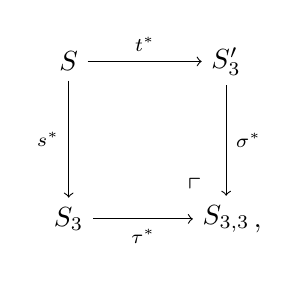
\begin{tikzpicture}
        \node (LT) at (0, 2) {$S$}; 
	\node (RT) at (2, 2) {$S_3'$}; 
        \node (LB) at (0, 0) {$S_3$}; 
	\node (RB) at (2, 0) {$S_{3,3}$}; 
	\node at (2.4, -0.125) {,}; 
	\node at (1.6, 0.4) {$\ulcorner$}; 
	\draw [->] (LT) -- node [above] {$\scriptstyle t^*$} (RT); 
	\draw [->] (LT) -- node [left] {$\scriptstyle s^*$} (LB); 
	\draw [->] (RT) -- node [right] {$\scriptstyle \sigma^*$} (RB); 
	\draw [->] (LB) -- node [below] {$\scriptstyle \tau^*$} (RB); 
\end{tikzpicture}
\end{center}
where $s^*$ is the inclusion, and $t^*$ sends $a$ to $a'$.  
Then $\sigma^*$ is the inclusion, and $\tau^*$ sends $a$ to $a'$, and $\A$ to $\A'$; 
they classify the subgroup $G$ of $C$, and the subgroup $G'$ of $C'$, respectively.  
Thus, via the evident isomorphism $S_3' \cong S_3$, 
$S_{3,3}$ carries the universal example of a chain $G < C[3]$ of subgroups of $C$, 
with $|G| = |C[3]/G| = 3$.  

By base change we then have a commutative diagram of elliptic curves over $S_{3,3}$: 
\begin{center}
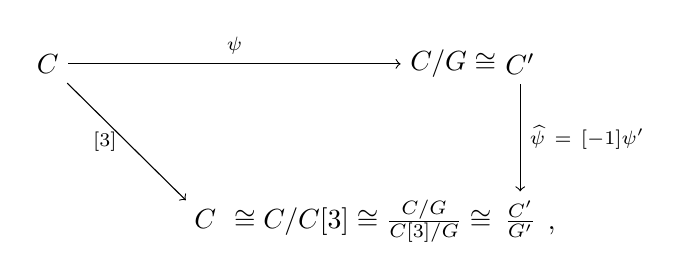
\begin{tikzpicture}
        \node (LT) at (0, 2) {$C$}; 
        \node (MT) at (5.15, 2) {$C/G \cong $}; 
        \node (RT) at (6, 2) {$C'$}; 
        \node (LB) at (2, 0.025) {$C$}; 
        \node (MB) at (4, 0) {$ \cong C/C[3] \cong \frac{C/G}{C[3]/G} \cong $}; 
        \node (RB) at (6, 0.025) {$\frac{C'}{G'}$}; 
	\node at (6.4, -0.125) {,}; 
        \draw [->] (LT) -- node [above] {$\scriptstyle \psi$} (MT);
        \draw [->] (LT) -- node [left] {$\scriptstyle [3]$} (LB); 
        \draw [->] (RT) -- node [right] {$\scriptstyle \widehat{\psi}~=~[-1] \psi'$} (RB); 
\end{tikzpicture}
\end{center}
where $\widehat{\psi}$ is the isogeny dual to $\psi$.  
Note that both $\psi$ and $\psi'$ restrict to the third-power Frobenius endomorphism $\psi_0$ over the supersingular locus.  
Since $\psi_0^2 = [-3]$ (\cff{5.11}{Y} and \cite[V.2.3.1]{AEC}), 
we have $\widehat{\psi} = [-1] \psi'$ by uniqueness of the dual isogeny (\cff{III.6.1a}{AEC}).  

The isogenies in the above diagram induce maps on relative cotangent spaces at the identity, 
and by proposition \ref{prop:isog} we have a commutative diagram 
\begin{equation}
\label{cotangent}
 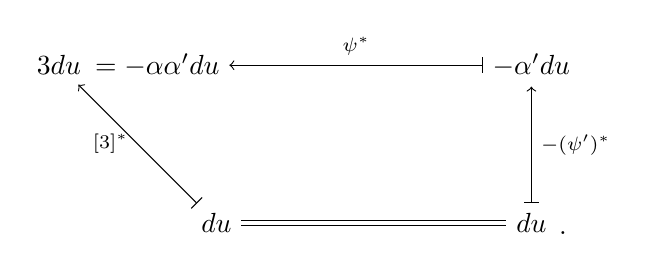
\begin{tikzpicture}[baseline=(current bounding box.center)]
         \node (LT) at (0, 2) {$3 du$}; 
         \node (MT) at (1.25, 2) {$= -\A \A' du$}; 
         \node (RT) at (6, 2) {$-\A' du$}; 
         \node (LB) at (2, 0) {$du$}; 
         \node (RB) at (6, 0) {$du$}; 
         \node at (6.4, -0.125) {.}; 
         \draw [|->] (RT) -- node [above] {$\scriptstyle \psi^*$} (MT);
         \draw [|->] (LB) -- node [left] {$\scriptstyle [3]^*$} (LT); 
         \draw [|->] (RB) -- node [right] {$\scriptstyle -(\psi')^*$} (RT); 
         \draw [double distance=1.3pt] (LB) -- (RB); 
 \end{tikzpicture}
\end{equation}

\begin{lem}
\label{lem:-p}
 The following relations hold in $S_{3,3}$: 
 \[
  \A \A' + 3 = 0, 
 \]
 and 
 \[
  \A' = -\A^3 + 6 \A + (-a^2 + 8).  
 \]
\end{lem}
\begin{proof}
 The first relation is read off from diagram \eqref{cotangent}.  From this and $w(\A) = 0$, we then get the second relation.  
\end{proof}

Let $S_9$ be the pullback in the diagram 
\begin{equation}
\label{S9}
 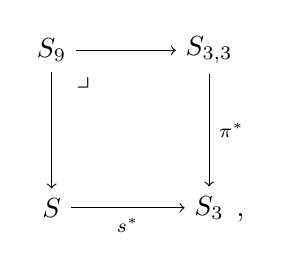
\begin{tikzpicture}[baseline=(current bounding box.center)]
         \node (LT) at (0, 2) {$S_9$}; 
         \node (RT) at (2, 2) {$S_{3,3}$}; 
         \node (LB) at (0, 0) {$S$}; 
         \node (RB) at (2, 0) {$S_3$}; 
         \node at (2.4, -0.125) {,}; 
         \node at (0.4, 1.6) {$\lrcorner$}; 
         \draw [->] (LT) --  (RT); 
         \draw [->] (LT) --  (LB); 
         \draw [->] (RT) -- node [right] {$\scriptstyle \pi^*$} (RB); 
         \draw [->] (LB) -- node [below] {$\scriptstyle s^*$} (RB); 
 \end{tikzpicture}
\end{equation}
where $\pi^*$ sends $a$ to $a$, $\A$ to $\A$, $a'$ to $r(a)$, and $\A'$ to $-\A^3 + 6 \A + (-a^2 + 8)$ as in lemma \ref{lem:-p}; 
it classifies the chain of subgroups $G < C[3]$ in $C$.  Thus the universal example of an order 9 subgroup of $C$ 
is defined over $S_9$, and the map $S_9 \to S$ classifies $C[3]$.  

Let $A$ be a $K(2)$-local commutative $E$-algebra.  
From the total power operation on $E_0$ in section \ref{sec:psi}, we have total power operations 
\[
 \p \co A_0 \to A_0 \otimes_{E_0} (E^0 B\Sigma_3 / I) \cong A_0 [\A] \big/ \big( w(\A) \big), 
\]
and 
\[
 \p \circ \p \co A_0 \to \big( A_0 \otimes_{E_0} (E^0 B\Sigma_3 / I) \big) \tensor[_{\scriptscriptstyle{\p}}]{\otimes}{_{E_0}} (E^0 B\Sigma_3 / I) 
\]
\[
 ~~~~~~~~~~~~~~~~~~~~~~~~~~~~~~~~~~~~~~~~\cong \Big( A_0 [\A'] \big/ \big( w'(\A') \big) \Big) \tensor[_{\scriptscriptstyle{\p}}]{\otimes}{_{E_0}} \Big( E^0 [\A] \big/ \big( w(\A) \big) \Big), 
\]
where $\A' = \p(\A) = -\A^3 + 6 \A + (-h + 12)$ by lemma \ref{lem:-p}.  

Define the {\em individual power operations} 
\[
 Q_i \co A_0 \to A_0, 
\]
for $i = 0, 1, 2, 3$, by 
\[
 \p (x) = Q_0(x) + Q_1(x) \A + Q_2(x) \A^2 + Q_3(x) \A^3.  
\]

\begin{prop}
\label{prop:Gamma}
 The following relations hold among the individual power operations $Q_0$, $Q_1$, $Q_2$, and $Q_3$: 
 \begin{enumerate}[(i)]
  \item Additivity 

  $Q_i(x+y) = Q_i(x) + Q_i(y)$; 

  \item Action on scalars 
  
  $Q_0(1) = 1$, 

  $Q_1(1) = Q_2(1) = Q_3(1) = 0$, 

  $Q_0(h) = h^3 - 36 h^2 + 390 h - 1212$, 

  $Q_1(h) = -6 h^2 + 144 h - 712$, 

  $Q_2(h) = 3 h - 36$, 

  $Q_3(h) = h^2 - 24 h + 120$, 

  $Q_0(a) = a^3 - 12 a + 12 a^{-1}$, 

  $Q_1(a) = -6 a + 20 a^{-1}$, 

  $Q_2(a) = 4 a^{-1}$, 

  $Q_3(a) = a - 4 a^{-1}$; 

  \item Commutation relations (twists) 

  $Q_0(h x) = (h^3 - 36 h^2 + 390 h - 1212) Q_0(x) + (3 h^2 - 72 h + 360) Q_1(x) + (9 h - 108) Q_2(x) + 24 Q_3(x)$, 

  $Q_1(h x) = (-6 h^2 + 144 h - 712) Q_0(x) + (-18 h + 228) Q_1(x) + (-72) Q_2(x) + (h - 12) Q_3(x)$, 

  $Q_2(h x) = (3 h - 36) Q_0(x) + 8 Q_1(x) + 12 Q_2(x) + (-24) Q_3(x)$, 

  $Q_3(h x) = (h^2 - 24 h + 120) Q_0(x) + (3 h - 36) Q_1(x) + 8 Q_2(x) + 12 Q_3(x)$, 

  $Q_0(a x) = (a^3 - 12 a + 12 a^{-1}) Q_0(x) + (3 a - 12 a^{-1}) Q_1(x) + (12 a^{-1}) Q_2(x) + (-12 a^{-1}) Q_3(x)$, 

  $Q_1(a x) = (-6 a + 20 a^{-1}) Q_0(x) + (-20 a^{-1}) Q_1(x) + (- a + 20 a^{-1}) Q_2(x) + (4 a - 20 a^{-1}) Q_3(x)$, 

  $Q_2(a x) = (4 a^{-1}) Q_0(x) + (-4 a^{-1}) Q_1(x) + (4 a^{-1}) Q_2(x) + (- a - 4 a^{-1}) Q_3(x)$, 

  $Q_3(a x) = (a - 4 a^{-1}) Q_0(x) + (4 a^{-1}) Q_1(x) + (-4 a^{-1}) Q_2(x) + (4 a^{-1}) Q_3(x)$; 

  \item Adem relations (products) 

  $Q_1Q_0(x) = (-6) Q_0Q_1(x) + (6 h - 72) Q_0Q_2(x) + (-6 h^2 + 144 h - 747) Q_0Q_3(x) + 18 Q_1Q_2(x) + 3 Q_2Q_1(x) + (-18 h + 216) Q_1Q_3(x) + (-54) Q_2Q_3(x) + (-9) Q_3Q_2(x)$, 

  $Q_2Q_0(x) = (-3) Q_0Q_2(x) + (3 h - 36) Q_0Q_3(x) + 9 Q_1Q_3(x) + 3 Q_3Q_1(x)$, 

  $Q_3Q_0(x) = Q_0Q_1(x) + (-h + 12) Q_0Q_2(x) + (h^2 - 24 h + 126) Q_0Q_3(x) + (-3) Q_1Q_2(x) + (3 h - 36) Q_1Q_3(x) + 9 Q_2Q_3(x)$; 

  \item Cartan formulas (coproducts) 

  $Q_0(xy) = Q_0(x) Q_0(y) + 3 \big(Q_1(x) Q_3(y) + Q_2(x) Q_2(y) + Q_3(x) Q_1(y)\big) + 18 Q_3(x) Q_3(y)$, 

  $Q_1(xy) = \big(Q_0(x) Q_1(y) + Q_1(x) Q_0(y)\big) + (-h + 12) \big(Q_1(x) Q_3(y) + Q_2(x) Q_2(y) + Q_3(x) Q_1(y)\big) + 3 \big(Q_2(x) Q_3(y) + Q_3(x) Q_2(y)\big) + (-6h + 72) Q_3(x) Q_3(y)$, 

  $Q_2(xy) = \big(Q_0(x) Q_2(y) + Q_1(x) Q_1(y) + Q_2(x) Q_0(y)\big) + 6 \big(Q_1(x) Q_3(y) + Q_2(x) Q_2(y) + Q_3(x) Q_1(y)\big) + (-h + 12) \big(Q_2(x) Q_3(y) + Q_3(x) Q_2(y)\big) + 39 Q_3(x) Q_3(y)$, 

  $Q_3(xy) = \big(Q_0(x) Q_3(y) + Q_1(x) Q_2(y) + Q_2(x) Q_1(y) + Q_3(x) Q_0(y)\big) + 6 \big(Q_2(x) Q_3(y) + Q_3(x) Q_2(y)\big) + (-h + 12) Q_3(x) Q_3(y)$; 

  \item Frobenius congruence (amplification) 

  $Q_0(x) \equiv x^3 \md 3$, 

  with $\theta \co A_0 \to A_0$ such that $Q_0(x) = x^3 + 3 \theta(x)$.  
 \end{enumerate}
\end{prop}
\begin{proof}
 Except for (iv), all the relations can be derived directly from corollary \ref{cor:psi3} and the fact that $\p$ is a ring homomorphism.  

 Write $\HS'$, $\HS_3'$, $\HS_{3,3}$, and $\HS_9$, analogous to $\HS_3$, to denote the completions of rings.  
 To derive (iv), we note that in view of diagram \eqref{S9} the composite 
 \[
  A_0 \stackrel{\p}{\to} A_0 \tensor[]{\otimes}{_{\HS}_{~s^*}} \HS_3 
  \stackrel{\p}{\to} A_0 \tensor[]{\otimes}{_{\HS'}_{~s^*}} \HS_3' \tensor[_{t^*}]{\otimes}{_{\HS}_{~s^*}} \HS_3 
  \cong A_0 \tensor[]{\otimes}{_{\HS}_{~s^*}} \HS_{3,3} 
 \]
 factors through $A_0 \otimes_{\HS} \HS_9$.  In terms of formulas we have 
 \begin{eqnarray*}
  \p \big( \p(x) \big) & = & \p \big( Q_0(x) + Q_1(x) \A + Q_2(x) \A^2 + Q_3(x) \A^3 \big) \\
                       & = & \p \big( Q_0(x) \big) + \p \big( Q_1(x) \big) \A' + \p \big( Q_2(x) \big) (\A')^2 + \p \big( Q_3(x) \big) (\A')^3 \\
                       & = & \sum_{i,~j~=~0}^3 Q_iQ_j(x) \A^i \big( -\A^3 + 6 \A + (-h + 12) \big)^j; 
 \end{eqnarray*}
 the factorization means that under the projection $\pi^* \co \HS_{3,3} \to \HS_3$ the coefficients of $\A$, $\A^2$, and $\A^3$ in the last expression must be 0 
 ($\A$ satisfies a quartic equation in $\HS_3$).  This gives the three relations in (iv).
\end{proof}

\begin{defn}
\label{def}
 We define an associative ring $\G$ equipped with a ring homomorphism 
 \footnote{The ring homomorphism $\eta$ is formally the inclusion: an element $s \in \HS = E_0$ maps to the multiplication-by-$s$ operation on the $E_0$-algebra $A_0$.  
 For precise definition of $\eta$, \cff{section 6}{cong}.  } $\eta \co \HS \to \G$ as follows.  
 The ring $\G$ is generated over $\HS$ by elements $Q_0$, $Q_1$, $Q_2$, and $Q_3$, subject to {\em commutation relations} and {\em Adem relations}.  
 The commutation relations state that the $Q_i$'s commute with elements of $\BZ_9 \subset \HS$, and that 

 $Q_0 h = (h^3 - 36 h^2 + 390 h - 1212) Q_0 + (3 h^2 - 72 h + 360) Q_1 + (9 h - 108) Q_2 + 24 Q_3$, 

 $Q_1 h = (-6 h^2 + 144 h - 712) Q_0 + (-18 h + 228) Q_1 + (-72) Q_2 + (h - 12) Q_3$, 

 $Q_2 h = (3 h - 36) Q_0 + 8 Q_1 + 12 Q_2 + (-24) Q_3$, 

 $Q_3 h = (h^2 - 24 h + 120) Q_0 + (3 h - 36) Q_1 + 8 Q_2 + 12 Q_3$.  

 The Adem relations are 

 $Q_1Q_0 = (-6) Q_0Q_1 + (6 h - 72) Q_0Q_2 + (-6 h^2 + 144 h - 747) Q_0Q_3 + 18 Q_1Q_2 + 3 Q_2Q_1 + (-18 h + 216) Q_1Q_3 + (-54) Q_2Q_3 + (-9) Q_3Q_2$, 

 $Q_2Q_0 = (-3) Q_0Q_2 + (3 h - 36) Q_0Q_3 + 9 Q_1Q_3 + 3 Q_3Q_1$, 

 $Q_3Q_0 = Q_0Q_1 + (-h + 12) Q_0Q_2 + (h^2 - 24 h + 126) Q_0Q_3 + (-3) Q_1Q_2 + (3 h - 36) Q_1Q_3 + 9 Q_2Q_3$.  
\qed
\end{defn}

\begin{rmk}
\label{rmk:rank}
 Proposition \ref{prop:Gamma} describes explicitly the structure of $\G$ as a {\em graded twisted bialgebra} over $E_0 = \HS$ (\cff{section 5}{cong} and \cite[2.1]{h2p2}).  
 In particular it follows that $\G$ has an {\em admissible basis}, that is, it is free as a left $\HS$-module on the elements of the form 
 \[
  Q_0^i Q_{k_1} \cdots Q_{k_r}, 
 \]
 where $i, r \geq 0$, and $k_j = 1, 2,$ or 3.  
 Note that if we write $\G[d]$ for the degree $d$ part of $\G$, then $\G[d]$ is of rank $1 + 3 + \cdots + 3^d$.  
\qed
\end{rmk}

\begin{exam}
\label{ex:omega}
 We have $E^0 S^2 \cong \BZ_9 \llbracket h \rrbracket [u] / (u^2)$.  
 By definition of $\A$ in \eqref{u'v'}, the $Q_i$'s act canonically on $E^0 S^2$: 
 \[
  Q_i \cdot u = \left\{
  \begin{array}{ll}
    u,  & \quad \text{if $i = 1$, }\\
    0,  & \quad \text{if $i \neq 1$.  }\\
  \end{array}
  \right.
 \]
 Let $\omega$ be the kernel of $E^0 S^2 \to E^0$.  It is a {\em $\G$-module} (\cff{2.2}{h2p2}) on one generator $u$, and its $\G$-module structure is canonical.  
\qed
\end{exam}

Following terminology in \cite[section 2]{cong} and \cite[2.5 and 2.6]{h2p2}, we can now describe the power operation structure on $K(2)$-local commutative $E$-algebras.  
\begin{thm}
\label{thm}
 Let $A$ be a $K(2)$-local commutative $E$-algebra.  
 Let $\G$ be the graded twisted bialgebra over $E_0$ given in definition \ref{def}, and let $\omega$ be the $\G$-module given in example \ref{ex:omega}.  
 Then $A_*$ is an {\em $\omega$-twisted $\BZ/2$-graded amplified $\G$-ring}.  In particular, 
 \[
  \pi_* L_{K(2)} \BP_E (\Sigma^d E) ~ \cong ~ {F_d}~_{(3,h)}^{\wedge} ~ , 
 \]
 where $F_d$ is the free $\omega$-twisted $\BZ/2$-graded amplified $\G$-ring on one generator in degree $d$.  
\end{thm}
Formulas of $\G$ aside, this result is essentially due to Rezk \cite{cong, h2p2}.  
\begin{proof}
 Let $\TG$ be the graded twisted bialgebra of power operations on $E$ described in \cite[section 6]{cong}.  
 It suffices to identify $\TG$ with $\G$.  
 There is a direct sum decomposition $\TG = \bigoplus_{d \geq 0} \TG[d]$, where the pieces come from the $E$-homology of $B\Sigma_{3^d}$ (\cff{6.2}{cong}).  
 There is a degree-preserving ring homomorphism $\phi \co \G \to \TG$ which is an isomorphism in degrees 0 and 1 (cf.\thinspace{c}orollary \ref{cor:psi3}).  
 As $\TG$ is generated in degree 1 (by transfer argument), $\phi$ is surjective.  
 By rank calculations (\cff{section 6}{ST} and remark \ref{rmk:rank}), $\phi$ is also injective.  
\end{proof}


\section{$K(1)$-local power operations}
\label{sec:K(1)}

Let $F = L_{K(1)} E$.  The general pattern of the relationship between $K(1)$-local power operations (\cf{K(1)E_infty}) 
and the power operations in section \ref{sec:psi} is as follows: 
\begin{center}
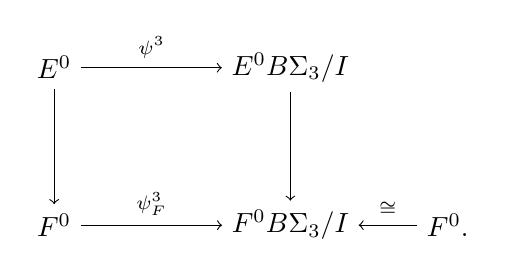
\begin{tikzpicture}
        \node (LT) at (0, 2) {$E^0$}; 
        \node (RT) at (3, 2) {$E^0 B\Sigma_3 / I$}; 
        \node (LB) at (0, 0) {$F^0$}; 
        \node (MB) at (3, 0) {$F^0 B\Sigma_3 / I$}; 
        \node (RB) at (5, 0) {$F^0.$}; 
        \draw [->] (LT) -- node [above] {$\scriptstyle \p$} (RT); 
        \draw [->] (LT) -- (LB); 
        \draw [->] (RT) -- (MB); 
        \draw [->] (LB) -- node [above] {$\scriptstyle \psi_F^3$} (MB); 
        \draw [->] (RB) -- node [above] {$\scriptstyle \cong$} (MB); 
\end{tikzpicture}
\end{center}
Recall proposition \ref{prop:isog} and corollary \ref{cor:psi3} that $\p$ arises from the universal degree 3 isogeny 
which is represented by the ring $S_3$ with $\HS_3 \cong E^0 B\Sigma_3 / I$.  The 
vertical maps are induced by the $K(1)$-localization $E \to F$.  In terms of 
homotopy groups, this is obtained by inverting the generator $h$ (so that 
the resulting formal group is of height at most 1) and completing at the ideal 
$(3)$, i.e.\thinspace$E_* = \BZ_9 \llbracket h \rrbracket [u^{\pm1}]$ and $F_* = \BZ_9 \llbracket h \rrbracket [h^{-1}]_3^\wedge [u^{\pm1}]$.  
Explicitly, 
\[
 F_0 = \BZ_9 (\!(h)\!)_3^\wedge = \varprojlim_k \BZ_9 (\!(h)\!) /(3^k) = 
 \left.\left\{\sum_{n = -\infty}^{\infty} c_n h^n~\right|~c_n \in \BZ_9, 
 \lim_{n \to -\infty} c_n = 0\right\}.  
\]
The formal group $\HC$ over $E^0$ has a unique order 3 subgroup after being pulled back to $F^0$ (cf.\thinspace{r}emark \ref{rmk:dmod3}), 
and the composite map $E^0 B\Sigma_3 / I \to F^0 B\Sigma_3 / I \cong F^0$ classifies this subgroup.  
The localization $E^0 B\Sigma_3 / I \to F^0 B\Sigma_3 / I$ factors through $F^0 \otimes_{E^0} E^0 B\Sigma_3 / I$.  
Along the base change $E^0 B\Sigma_3 / I \to F^0 \otimes_{E^0} E^0 B\Sigma_3 / I$, 
the special fiber of the 3-divisible group $\HC$ which consists solely of a formal component may split into formal and \'etale components.  
We want to take the formal component so as to keep track of the unique order 3 subgroup of the formal group over $F^0$ 
which gives rise to the $K(1)$-local power operation $\psi_F^3$.  

In proposition \ref{prop:isog} the equation 
\[
 w(\A) = \A^4 - 6 \A^2 + (h - 12) \A - 3 = 0 
\]
which parametrizes order 3 subgroups of $C$ has a unique root 
in $\BF_3 (\!(h)\!)$, and Hensel's lemma implies that this lifts to a 
root in $F_0 = \BZ_9 (\!(h)\!)_3^\wedge$.  Plugging this 
specific value of $\A$ into the formulas of $\p \co E^0 \to E^0 [\A] \big/ \big( w(\A) \big)$ given in corollary \ref{cor:psi3}, we 
get an endomorphism of the ring $F_0$, and this endomorphism is $\psi_F^3$.  

Explicitly, with $h$ invertible in $F_0$, we can solve for $\A$ from the equation $w(\A) = 0$ by first writing 
\[
 \A = \frac{1}{h - 12} (3 + 6 \A^2 - \A^4) = (3 + 6 \A^2 - \A^4) \cdot \sum_{n = 1}^\infty 12^{n-1} h^{-n} 
\]
and then substituting $\A$ recursively.  We plug this into $\p(h)$ and get 
\[
 \psi_F^3(h) = h^3 - 36 h^2 + 372 h - 996 + 186 h^{-1} + 2232 h^{-2} + \cdots.  
\]
Similarly we have 
\[
 \psi_F^3(a) = a^3 - 12 a - 6 a^{-1} - 84 a^{-3} - 933 a^{-5} - 10956 a^{-7} + \cdots.  
\]

For an application of the analogous calculations at the prime 2, see \cite[section 8.2]{level3}.  


\newpage

%\nocite{*}
%\bibliographystyle{amsalpha}
%\bibliography{p3}
%\end{document}

\newcommand{\MRn}[2]{\href{http://www.ams.org/mathscinet-getitem?mr=#1}{MR#1} #2}
\begin{thebibliography}

\bibitem[AHS01]{cube}
M.~Ando, M.~J. Hopkins, and N.~P. Strickland, \emph{Elliptic spectra, the
  {W}itten genus and the theorem of the cube}, Invent. Math. \textbf{146}
  (2001), no.~3, 595--687. \MRn{1869850}{(2002g:55009)}

\bibitem[BMMS86]{H_infty}
R.~R. Bruner, J.~P. May, J.~E. McClure, and M.~Steinberger, \emph{{$H\sb \infty
  $} ring spectra and their applications}, Lecture Notes in Mathematics, vol.
  1176, Springer-Verlag, Berlin, 1986. \MRn{836132}{(88e:55001)}

\bibitem[BW05]{BW}
James Borger and Ben Wieland, \emph{Plethystic algebra}, Adv. Math.
  \textbf{194} (2005), no.~2, 246--283. \MRn{2139914}{(2006i:13044)}

\bibitem[EKMM97]{EKMM}
A.~D. Elmendorf, I.~Kriz, M.~A. Mandell, and J.~P. May, \emph{Rings, modules,
  and algebras in stable homotopy theory}, Mathematical Surveys and Monographs,
  vol.~47, American Mathematical Society, Providence, RI, 1997, With an
  appendix by M. Cole. \MRn{1417719}{(97h:55006)}

\bibitem[Gre88]{blind}
J.~P.~C. Greenlees, \emph{How blind is your favourite cohomology theory?},
  Exposition. Math. \textbf{6} (1988), no.~3, 193--208. \MRn{949783}{(89j:55001)}

\bibitem[Hop]{K(1)E_infty}
M.~J. Hopkins, \emph{K(1)-local ${E}_\infty$ ring spectra}, available at
  \url{http://www.math.rochester.edu/u/faculty/doug/otherpapers/knlocal.pdf}.

\bibitem[LN]{level3}
Tyler Lawson and Niko Naumann, \emph{Commutativity conditions for truncated
  {B}rown-{P}eterson spectra of height 2}, \href{http://arxiv.org/abs/1101.3897}{arXiv:1101.3897}.

\bibitem[Reza]{lpo}
Charles Rezk, \emph{Lectures on power operations}, available at
  \url{http://www.math.uiuc.edu/~rezk/power-operation-lectures.dvi}.

\bibitem[Rezb]{h2p2}
\bysame, \emph{Power operations for {M}orava ${E}$-theory of height 2 at the
  prime 2}, \href{http://arxiv.org/abs/0812.1320}{arXiv:0812.1320}.

\bibitem[Rez09]{cong}
\bysame, \emph{The congruence criterion for power operations in {M}orava
  {$E$}-theory}, Homology, Homotopy Appl. \textbf{11} (2009), no.~2, 327--379.
  \MRn{2591924}{(2011e:55021)}

\bibitem[Sil09]{AEC}
Joseph~H. Silverman, \emph{The arithmetic of elliptic curves}, second ed.,
  Graduate Texts in Mathematics, vol. 106, Springer, Dordrecht, 2009.
  \MRn{2514094}{(2010i:11005)}

\bibitem[ST97]{ST}
Neil~P. Strickland and Paul~R. Turner, \emph{Rational {M}orava {$E$}-theory and
  {$DS\sp 0$}}, Topology \textbf{36} (1997), no.~1, 137--151. \MRn{1410468}{(97g:55005)}

\bibitem[Ste62]{steenrod}
N.~E. Steenrod, \emph{Cohomology operations}, Lectures by N. E. Steenrod
  written and revised by D. B. A. Epstein. Annals of Mathematics Studies, No.
  50, Princeton University Press, Princeton, N.J., 1962. \MRn{0145525}{(26
  \#3056)}

\bibitem[Str98]{Str98}
N.~P. Strickland, \emph{Morava {$E$}-theory of symmetric groups}, Topology
  \textbf{37} (1998), no.~4, 757--779. \MRn{1607736}{(99e:55008)}

\bibitem[Voe03]{V}
Vladimir Voevodsky, \emph{Reduced power operations in motivic cohomology},
  Publ. Math. Inst. Hautes \'Etudes Sci. (2003), no.~98, 1--57. \MRn{2031198}{(2005b:14038a)}

\bibitem[Yui79]{Y}
Noriko Yui, \emph{Formal groups and some arithmetic properties of elliptic
  curves}, Algebraic geometry ({P}roc. {S}ummer {M}eeting, {U}niv.
  {C}openhagen, {C}openhagen, 1978), Lecture Notes in Math., vol. 732,
  Springer, Berlin, 1979, pp.~630--658. \MRn{555721}{(80m:14027)}

\end{thebibliography}
\end{document}